\documentclass[conference]{IEEEtran}

\usepackage{cite}
\usepackage{amsmath,amssymb}
\usepackage{booktabs}
\usepackage{array}
\usepackage{url}
\usepackage{graphicx}
\usepackage{tikz}
\usepackage{float}
\usepackage{afterpage}
\usetikzlibrary{shapes.geometric, arrows.meta, positioning}

\begin{document}

\title{An Explainable Heterogeneous Machine Learning and Deep Learning Framework for Early Diabetes Risk Prediction}

\author{
\IEEEauthorblockN{
Mrinal Singh,
Jagrati Sharma,
Sidhida Rath,
Mehul Jha,
Bhaswar Deep Rout
}
\IEEEauthorblockA{
Department of Computer Science and Engineering\\
Kalinga Institute of Industrial Technology\\
Bhubaneswar, India\\
Email: (2405739, 2405287, 24052261, 2405281, 2405868)@kiit.ac.in
}
}

\maketitle

\begin{abstract}
Diabetes mellitus is a major chronic health condition in which early detection can reduce the risk of serious long-term complications. Machine learning and deep learning techniques have demonstrated significant potential for identifying individuals at risk from patient health indicators. However, challenges such as class imbalance, model complexity, limited interpretability, and potential data leakage can reduce the reliability and clinical usefulness of predictive systems. This study proposes an explainable heterogeneous machine learning and deep learning framework for early diabetes risk prediction. The framework evaluates multiple model families together with ensemble learning and Explainable Artificial Intelligence (XAI). The proposed pipeline incorporates systematic preprocessing, feature analysis, hyperparameter optimization, class-imbalance handling using SMOTE, and out-of-fold prediction-based stacking. A number of different heterogeneous models are evaluated based on accuracy, precision, recall, F1 score, ROC AUC, and various other criteria. The optimization and preprocessing are done based only on the training set without touching the test set at all. Out-of-fold predictions prevent training-label leakage in the ensemble, while SHAP identifies key features contributing to diabetes risk. The framework balances performance, reliability, and interpretability for trustworthy AI-based diabetes prediction.
\end{abstract}

\begin{IEEEkeywords}
Diabetes Prediction, Machine Learning, Deep Learning, Ensemble Learning, Stacking, SMOTE, Explainable Artificial Intelligence, SHAP, XGBoost
\end{IEEEkeywords}

\section{Introduction}

Diabetes mellitus is a long term metabolic disease that is characterized by abnormally high blood glucose levels that can lead to various complications over time such as cardiovascular disease, kidney disease, neuropathy, retinopathy. Identification of people at high risk for this disease in an early stage is important as it allows better disease management and timely interventions. Therefore, automated prediction systems based on patient health indicators have received increasing attention.

Machine learning (ML) is used to analyze healthcare data as it can identify complex patterns and relationships. Several traditional ML algorithms such as Logistic Regression, Random Forest, Support Vector Machine (SVM), and gradient boosting methods have been applied to diabetes prediction and they have shown favourable predictive performance. More recently, deep learning (DL) models have been explored as they have the ability to learn complex patterns from data, can model nonlinear relationships and can capture interactions between different features.

Even though the ML models can provide good predictions they still face challenges when applied to healthcare data. Diabetes datasets can contain class imbalance, usually where the number of non-diabetic observations exceeds diabetic observations. When such imbalances are encountered a model may become biased towards the majority class (non diabetic class) consequently reducing recall for the diabetic class.

Furthermore, highly complex models may behave as black boxes. This lack of interpretability can reduce confidence in using ML predictions in the healthcare environment. Explainable Artificial Intelligence (XAI) addresses this issue by providing information about how the model arrives at its prediction thus improving the transparency of ML systems.

SHapley Additive exPlanations (SHAP), one of the available techniques, estimates the contribution of individual features in the prediction. It can indicate whether particular features have a stronger influence on the model's output hence helping the user understand the relationship between input features and predictions.

Another concern is methodological reliability. Preprocessing, oversampling, hyperparameter tuning, threshold selection, and ensemble construction can cause leakage of information while validating or when the test data are used. A reliable framework should keep training separate from the final test evaluation.

The objective is to develop a reproducible diabetes prediction framework combining heterogeneous Machine Learning and Deep Learning models with ensemble learning and XAI. The methodology focuses on preprocessing, hyperparameter optimization, SMOTE experiments, out-of-fold stacking, leakage-free threshold selection, and SHAP-based interpretation.

\section{Literature Review}

More advanced ensemble architectures have been explored. In
\cite{ELGENDY2025126899}, a dual-stage explainable stacking framework was proposed using seven base learners: AdaBoost, Gradient Boosting, Histogram Gradient Boosting, Extra Trees, CatBoost, XGBoost, and KNN. The framework incorporated autoencoder-based reconstruction, multiple imputation strategies, and SMOTE, with Bagging, Random Forest, MLP, and Logistic Regression as meta-models. Feature importance and SHAP were used for explainability. The framework was evaluated on MIMIC-IV and Pima Indians Diabetes datasets, demonstrating the potential of stacking for robust and interpretable diabetes prediction.

In \cite{netayawijit2025}, class imbalance in diabetes prediction was addressed by integrating SMOTE with SHAP and evaluating Random Forest, Gradient Boosting, SVM, Logistic Regression, and XGBoost. SMOTE and preprocessing were applied within the training folds of 5-fold stratified cross-validation to prevent data leakage. The study highlights the importance of leakage-aware evaluation for imbalanced datasets and the need for validation on larger and more diverse datasets.

In \cite{PANG2025100390}, explainable machine learning for diabetes prediction was studied using six ML models and the Multivariate
Adaptive Regression Splines (MARS) model on a large CDC dataset. SHAP was used to explain feature importance and individual predictions, while MARS provided an explicit mathematical relationship between input features and diabetes risk, enabling what-if analysis. The study identified General Health, High Blood Pressure, Age, BMI, and High Cholesterol as the most influential features.

In \cite{islam2025}, an explainable diabetes prediction framework was proposed integrating preprocessing,random oversampling, and hyperparameter tuning with KNN, Random Forest, Decision Tree, and Extra Trees. The study used the BRFSS and Diabetes 2019 datasets, with GridSearchCV for optimization and SHAP, LIME, and PDP for explainability. Extra Trees achieved the best performance, with 97.23\% accuracy on BRFSS and 97.45\% on Diabetes 2019. However, the study focuses mainly on individual conventional machine learning classifiers rather than ensemble or hybrid deep learning architectures.

In \cite{aulia2025}, an optimized Random Forest classifier with SHAP was used on the Pima Indians Diabetes Dataset to compare SMOTE and
ADASYN. ADASYN performed best, achieving 82.01\% accuracy, 70.91\% precision, 81.25\% recall, and 75.73\% F1-score. Glucose, BMI, and Age were the most influential features across sampling methods. The results show that oversampling can improve performance while maintaining consistent feature importance.

In \cite{Kibria2022}, a soft voting ensemble framework for diabetes prediction was proposed by combining Naïve Bayes, Logistic Regression, and Random Forest. To improve the interpretability of the model, SHAP and LIME were incorporated to explain the contribution of individual features to the predictions, demonstrating the value of explainable ensemble learning.

In \cite{Ganguly2023}, an ensemble learning framework was proposed that combined multiple machine learning classifiers with SHAP and LIME. The work focused on understanding the relationships between input features and model predictions, thereby improving the interpretability and transparency of the diabetes prediction process.

In \cite{Islam2025EarlyDiabetes}, an Explainable Ensemble Learning Framework (EELF) was introduced that incorporated feature engineering, feature selection, and a voting-based ensemble classifier. SHAP and LIME were integrated to improve model interpretability and support early-stage diabetes prediction.

In \cite{Islam2025Performance}, an ensemble framework was proposed combining Random Forest, XGBoost, and LightGBM. To enhance interpretability, the framework incorporated SHAP, LIME, Partial Dependence Plots (PDP), and Individual Conditional Expectation (ICE) to explain model predictions.

In \cite{rafie2025}, a Type 2 diabetes prediction framework was proposed using XGBoost and CatBoost after preprocessing the data. Feature selection was performed using LightGBM, class balancing was performed using SMOTE, and hyperparameter tuning and 10-fold cross-validation were applied. SHAP was used to interpret both overall and individual model predictions. The findings demonstrate the effectiveness of optimized gradient boosting algorithms for structured clinical data and highlight the potential of XGBoost and CatBoost for diabetes risk prediction. But the study was mainly focused on boosting based machine learning algorithms like XGBoost and CatBoost. While other approaches like deep learning models and hybrid ensemble methods were not evaluated. Furthermore, the model was validated on a specific population and requires further validation on different datasets representing diverse populations.

In \cite{zaferani2026}, a transparent hybrid framework was presented by combining Random Forest, K-Nearest Neighbors, and Neural Networks using stacking and voting ensemble strategies. SHAP and LIME were used to explain model predictions, both globally and locally. The study shows that combining heterogeneous learning models, ensemble techniques and explainable artificial intelligence can improve transparency in diabetes prediction. However, future work should consider advanced hybrid architectures, extensive model comparison, robust validation on a variety of datasets and clinically reliable evaluation frameworks.

LIME-based explanations were also used to study patient-level diabetes prediction \cite{khokhar2025}. The study demonstrated that LIME can generate local explanations for individual predictions by highlighting patient features that affect the model outputs. However, the reliability of LIME explanations may vary depending on dataset characteristics, as their fidelity can differ across datasets. Therefore, further evaluation and comparison with multiple XAI techniques are required to ensure trustworthy explanations.

There is also growing interest in the reliability of explanations
themselves. In \cite{arora2025}, different XAI techniques such as SHAP, LIME, Explainable Boosting Machines (EBM), and counterfactual explanations were compared, and the quality of explanations was evaluated using metrics such as fidelity, faithfulness, sparsity, stability, and consistency. The results suggest that different XAI techniques can provide different insights into model behavior of the underlying model and dataset. This work highlights that we should systematically evaluate the quality, fidelity and reliability of explanations, and reliability should be systematically evaluated, as interpretability alone does not guarantee trustworthy explanations.


Finally, \cite{masood2026} provided a systematic review of AI-powered approaches for diabetes prediction covering conventional machine learning, deep learning, ensemble learning, hybrid approaches, and explainable AI. The review demonstrated that ensemble techniques such as Random Forest and XGBoost perform well on structured clinical data, whereas deep learning models such as CNNs are well suited for medical imaging and LSTM/GRU networks are effective for time-series data such as continuous glucose monitoring. The review also highlights some challenges including class imbalance, interpretability, generalizability, computational requirements, data privacy and clinical deployment. These observations highlight the necessity of rigorous evaluation, careful validation, and reproducible approaches in diabetes prediction research.

Overall, the literature review indicated that ensemble learning, class balancing, model optimization, deep learning and explainable AI have advanced significantly in the prediction of diabetes. However, the research gap is not the absence of these techniques but their systematic integration and rigorous evaluation. Existing literature emphasizes the necessity of leakage-sensitive preprocessing, appropriate class balancing, hyperparameter tuning, strong ensemble construction, and evaluation using several metrics beyond accuracy. Based on these results, this work proposes a complete pipeline for diabetes prediction that comprises: (1) preprocessing of data, (2) comparison of machine learning and deep learning models, (3) hyperparameter optimization, (4) experiments with SMOTE, (5) out-of-fold stacking, (6) threshold optimization to avoid leakage, and (7) interpretation with SHAP, keeping an intact test set for the final evaluation. The framework aims at a trade-off between predictive performance, reliability and interpretability.



\section{Proposed Methodology}

% \subsection{Figure 1: Proposed Framework Flowchart}



\subsection{Overview of the Proposed Approach}

The proposed study develops an explainable machine learning framework for diabetes risk prediction using structured health-related attributes. The main objective is not only to obtain a strong predictive model but also to examine how the model arrives at its predictions. This is particularly important in a healthcare setting, where a prediction without an interpretable explanation may be difficult to evaluate or trust.

The complete methodology consists of several sequential stages. The process begins with dataset inspection and data-quality verification, followed by preprocessing and feature transformation. The processed dataset is then divided into training and testing subsets while maintaining the class distribution. Several machine learning models are trained to establish baseline performance. Additional experiments are performed using SMOTE to investigate the effect of class balancing, while hyperparameter tuning is applied to selected models to improve their predictive performance.

Following the individual model experiments, an out-of-fold stacking approach is developed using predictions from multiple base learners. The stacking model produces probability estimates rather than directly relying on a fixed classification boundary. A classification threshold is subsequently optimized using only the out-of-fold training predictions. This prevents information from the untouched test set from influencing the threshold-selection process.

Finally, the best-performing individual model is examined using SHAP-based explainability. This provides both a global view of feature importance and feature-level relationships that help explain the model's predictions.

The workflow proceeds from data validation and preprocessing to feature transformation, stratified splitting, comparative model development, SMOTE experiments, hyperparameter optimization, model comparison, OOF stacking, OOF threshold selection, final testing, and SHAP-based explainability.

\begin{figure*}[!t]
\centering

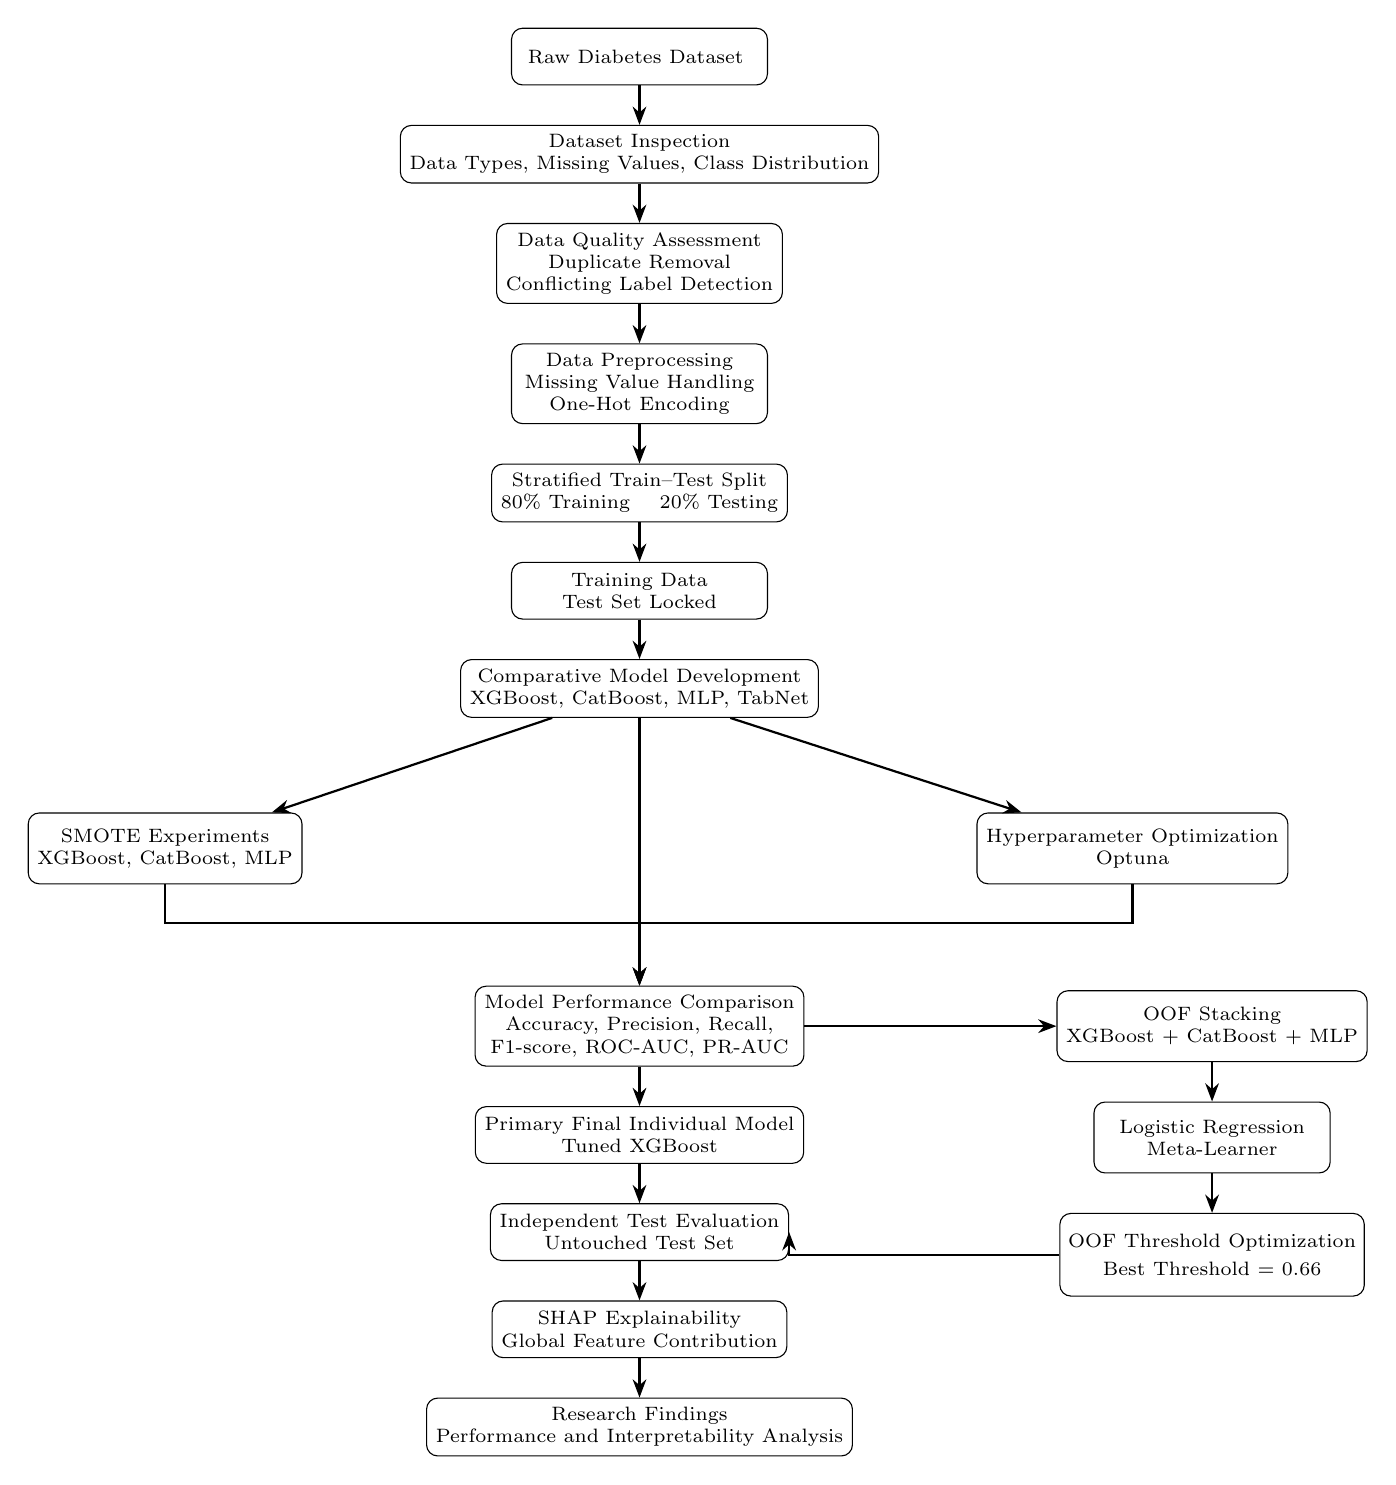
\begin{tikzpicture}[
    node distance=5mm and 10mm,
    transform shape,
    box/.style={
        rectangle,
        rounded corners,
        draw,
        align=center,
        minimum width=3.25cm,
        minimum height=0.72cm,
        font=\scriptsize
    },
    smallbox/.style={
        rectangle,
        rounded corners,
        draw,
        align=center,
        minimum width=3.0cm,
        minimum height=0.90cm,
        font=\scriptsize
    },
    arrow/.style={
        thick,
        -{Stealth}
    }
]

% ------------------------------------------------
% Main preprocessing pipeline
% ------------------------------------------------

\node[box] (raw) {
    Raw Diabetes Dataset
};

\node[box, below=of raw] (inspect) {
    Dataset Inspection\\
    Data Types, Missing Values, Class Distribution
};

\node[box, below=of inspect] (quality) {
    Data Quality Assessment\\
    Duplicate Removal\\
    Conflicting Label Detection
};

\node[box, below=of quality] (preprocess) {
    Data Preprocessing\\
    Missing Value Handling\\
    One-Hot Encoding
};

\node[box, below=of preprocess] (split) {
    Stratified Train--Test Split\\
    80\% Training \quad 20\% Testing
};

% ------------------------------------------------
% Training data
% ------------------------------------------------

\node[box, below=of split] (training) {
    Training Data\\
    Test Set Locked
};

\node[box, below=of training] (models) {
    Comparative Model Development\\
    XGBoost, CatBoost, MLP, TabNet
};

% ------------------------------------------------
% Experimental branches
% ------------------------------------------------

\node[smallbox, below left=12mm and 20mm of models] (smote) {
    SMOTE Experiments\\
    XGBoost, CatBoost, MLP
};

\node[smallbox, below right=12mm and 20mm of models] (tuning) {
    Hyperparameter Optimization\\
    Optuna
};

\node[box, below=34mm of models] (comparison) {
    Model Performance Comparison\\
    Accuracy, Precision, Recall,\\
    F1-score, ROC-AUC, PR-AUC
};

% ------------------------------------------------
% Stacking branch
% ------------------------------------------------

\node[smallbox, right=32mm of comparison] (oof) {
    OOF Stacking\\
    XGBoost + CatBoost + MLP
};

\node[smallbox, below=of oof] (meta) {
    Logistic Regression\\
    Meta-Learner
};

\node[smallbox, below=of meta, minimum height=1.05cm, inner sep=3pt] (threshold) {
    OOF Threshold Optimization\\[2pt]
    Best Threshold = 0.66
};

% ------------------------------------------------
% Final model branch
% ------------------------------------------------

\node[box, below=of comparison] (final) {
    Primary Final Individual Model\\
    Tuned XGBoost
};

\node[box, below=of final] (evaluation) {
    Independent Test Evaluation\\
    Untouched Test Set
};

\node[box, below=of evaluation] (shap) {
    SHAP Explainability\\
    Global Feature Contribution
};

\node[box, below=of shap] (findings) {
    Research Findings\\
    Performance and Interpretability Analysis
};

% ------------------------------------------------
% Arrows: main pipeline
% ------------------------------------------------

\draw[arrow] (raw) -- (inspect);
\draw[arrow] (inspect) -- (quality);
\draw[arrow] (quality) -- (preprocess);
\draw[arrow] (preprocess) -- (split);
\draw[arrow] (split) -- (training);
\draw[arrow] (training) -- (models);

% ------------------------------------------------
% Experimental branches
% ------------------------------------------------

\draw[arrow] (models) -- (smote);
\draw[arrow] (models) -- (tuning);


\draw[arrow] (smote.south)  |- ([yshift=8mm]comparison.north) -- (comparison.north);
\draw[arrow] (tuning.south) |- ([yshift=8mm]comparison.north) -- (comparison.north);
\draw[arrow] (models) -- (comparison);

% ------------------------------------------------
% Model selection and final evaluation
% ------------------------------------------------

\draw[arrow] (comparison) -- (final);
\draw[arrow] (final) -- (evaluation);
\draw[arrow] (evaluation) -- (shap);
\draw[arrow] (shap) -- (findings);

% ------------------------------------------------
% OOF stacking branch
% ------------------------------------------------

\draw[arrow] (comparison) -- (oof);
\draw[arrow] (oof) -- (meta);
\draw[arrow] (meta.south) -- (threshold.north);

% Threshold-selected stacking model evaluated
\draw[arrow] (threshold.west) -| (evaluation.east);

\end{tikzpicture}

\caption{
Complete workflow of the proposed explainable diabetes risk-prediction
framework. The methodology consists of data-quality assessment,
leakage-free preprocessing, stratified train--test partitioning,
comparative model development, separate SMOTE and hyperparameter
optimization experiments, model comparison, OOF stacking with a
Logistic Regression meta-learner, OOF-based threshold optimization,
independent test evaluation, and SHAP-based explainability.
The independent test set remains isolated from model development and
threshold selection.
}

\label{fig:workflow}

\end{figure*}

\subsection{Dataset Preparation and Data Quality Assessment}

The original dataset contains 100,000 observations and 9 attributes. Data quality checks identified and removed 3,854 duplicate rows and 182 observations belonging to 91 conflicting feature/target groups. After cleaning and categorical encoding, the final modeling dataset contains 95,964 observations and 16 features. The final audit reported zero missing values, duplicates, infinite values, conflicting observations, or identical feature patterns between training and testing.

A separate train/test overlap audit also found zero identical feature patterns.

\subsection{Data Preprocessing}


Numerical variables are retained in numerical form, while categorical variables such as gender and smoking history are one hot encoded. The binary target is represented as 0 for non-diabetic and 1 for diabetic observations. The preprocessing pipeline is applied consistently without allowing the test set to influence learned transformations.

\subsection{Class Distribution and Imbalance Handling}


An important characteristic of the dataset is the unequal distribution of the target classes. After data cleaning, the dataset contains 87,573 non-diabetic observations and 8,391 diabetic observations. Therefore, the positive class represents approximately 8.74\% of the final dataset.

This imbalance could be a potential problem for binary classification. A model can achieve high overall accuracy by biasing the majority class, even while missing a significant amount of diabetic cases. That is why accuracy is deemed to be inadequate as the sole measure of evaluation. Accuracy is considered together with Precision, Recall, F1-score, ROC-AUC and PR-AUC. In particular, recall gives information about the ability of the model to identify positive cases of diabetes and precision shows how many of the cases predicted to be diabetic are actually positive. We also conduct experiments based on SMOTE to check if explicit balancing of classes improves the predictive behaviour. These experiments are treated as different model configurations, instead of assuming that oversampling will automatically lead to better results.


\subsection{Training and Testing Strategy}

The final dataset is divided into training and testing subsets using a stratified split. The training portion contains 76,771 observations, while the test portion contains 19,193 observations. The stratified division preserves the relative distribution of the target classes in both subsets.

More importantly, the test subset is kept separate from model development and threshold optimization. The training data are used for model training, hyperparameter optimization, OOF prediction generation, stacking meta model construction, and classification threshold selection. The test data are reserved for final evaluation.

An additional train/test overlap audit was performed. The analysis found zero identical feature patterns between the training and testing sets, providing an additional check against unintended data overlap.
\subsection{Individual Machine Learning Models}

Four heterogeneous algorithms are evaluated: XGBoost and CatBoost as gradient-boosted tree learners, MLP as a neural-network alternative, and TabNet as a deep-learning architecture designed for tabular data. Baseline and tuned configurations are compared where applicable, while SMOTE versions are evaluated separately. This design provides a consistent comparison of tree ensembles and neural approaches rather than relying on a single model family.

\subsection{SMOTE-Based Experiments}

Because only 8.74\% of the observations belong to the positive class, Synthetic Minority Over-sampling Technique (SMOTE) is investigated as a separate experimental condition.

SMOTE generates synthetic minority-class observations based on existing minority samples. Rather than simply duplicating positive observations, it creates additional synthetic samples in the feature space.

In this study, SMOTE is evaluated with XGBoost, CatBoost, and MLP. The purpose is to determine whether increasing the representation of the minority class produces a useful improvement in diabetes detection.

An important aspect of the proposed methodology is that SMOTE is treated as an experiment rather than an assumed improvement. The resulting models are compared against their corresponding non-SMOTE configurations using the same evaluation criteria. This allows the study to determine whether balancing the training data actually improves the final predictive trade-off between precision and recall.

\subsection{Hyperparameter Optimization}

After establishing the baseline models, hyperparameter optimization is performed for XGBoost, CatBoost, and MLP.

Hyperparameters determine aspects of model behavior that are not learned directly from individual training observations. For example, tree-based models can be affected by parameters controlling tree complexity, learning rate, and ensemble size, whereas neural networks are affected by architectural and optimization parameters.

The tuning process searches for configurations that provide improved validation performance while avoiding dependence on the final test set. The tuned models are then evaluated alongside their baseline counterparts. This comparison makes it possible to determine whether the additional optimization provides a meaningful improvement.

Among the evaluated configurations, tuned XGBoost achieved the highest F1-score, ROC-AUC, and PR-AUC on the independent test set and was therefore selected as the primary final individual model.

\subsection{Model Selection}

Models are compared using accuracy, precision, recall, F1-score, ROC-AUC, and PR-AUC. Together these measures capture overall correctness, positive-prediction quality, sensitivity, the precision-recall balance, discrimination across thresholds, and precision-recall behavior under class imbalance.

\subsection{Proposed Stacking Ensemble}

In addition to evaluating individual models, the study investigates whether predictions from different learning algorithms can be combined through stacking.

The stacking framework uses the predictions of multiple base learners as inputs to a higher-level meta-model. In the proposed implementation, predictions from CatBoost, XGBoost, and MLP are used to construct the meta-level representation.

The important aspect of this process is the use of out-of-fold (OOF) predictions. Instead of generating predictions for a training observation using a model that has already seen that observation during training, the training data are divided into folds. Each observation receives a prediction from a model that was trained without that observation.

These predictions form the OOF meta-features. The resulting structure is therefore:

\begin{enumerate}
    \item Training Data
    \item Base Models
    \item OOF Predictions
    \item Meta-Model
    \item Stacking Probability
\end{enumerate}

This approach reduces the possibility that the meta-model simply learns predictions produced from data already seen by the base models.

\subsection{Leakage-Free Threshold Optimization}

The stacking model produces a probability for the positive class. A probability value must subsequently be converted into a binary prediction using a classification threshold. The conventional threshold of 0.50 is not necessarily optimal for an imbalanced medical prediction problem.

Therefore, the proposed framework determines an alternative threshold using the OOF predictions. Candidate thresholds ranging from 0.10 to 0.90, in increments of 0.01, are evaluated. For every candidate threshold, accuracy, precision, recall, and F1-score are calculated.

The threshold producing the highest OOF F1-score is selected.

\begin{equation}
\text{Best OOF Threshold} = 0.66
\end{equation}

\begin{equation}
\text{OOF F1-score} = 0.8135
\end{equation}

Most importantly, this threshold is selected exclusively from the training-side OOF predictions. The untouched test set is not used to search for the threshold.

After the threshold has been fixed at 0.66, it is applied once to the independent test probabilities to obtain the final stacking predictions. This procedure is referred to as leakage-free threshold optimization because the test labels do not participate in threshold selection.

\subsection{Final Model Evaluation}

The final evaluation is performed only after all model-development decisions have been completed.

For the selected tuned XGBoost model, the test-set results are accuracy 0.9716, precision 0.9757, recall 0.6925, F1-score 0.8100, ROC-AUC 0.9778, and PR-AUC 0.8855.

The corresponding confusion matrix contains 17,486 true negatives, 29 false positives, 516 false negatives, and 1,162 true positives.

The results indicate that the selected model provides strong overall discrimination while maintaining high precision. However, the recall value also shows that a proportion of positive cases remain unidentified. This limitation is important and should be explicitly acknowledged rather than presenting the model as error-free.

For comparison, the leakage-free stacking threshold experiment obtains accuracy 0.9711, precision 0.9554, recall 0.7020, F1-score 0.8093, ROC-AUC 0.9775, and PR-AUC 0.8853.

The stacking configuration therefore produces a slightly higher recall than the tuned XGBoost model but does not exceed the tuned XGBoost configuration in F1-score or ROC-AUC. Consequently, tuned XGBoost is selected as the primary final model, while the stacking experiment serves as an additional ensemble investigation within the proposed framework.

\subsection{Explainable Artificial Intelligence Using SHAP}

Predictive performance alone does not explain why a model generates a particular diabetes-risk prediction. To address this issue, the proposed methodology incorporates SHAP (SHapley Additive exPlanations) for model interpretation.

SHAP assigns contribution values to individual features for a prediction. These values indicate how each feature contributes toward increasing or decreasing the model output relative to the model's baseline prediction.

The explainability analysis is performed on the final tuned XGBoost model. Two levels of interpretation are considered.

\subsubsection{Global Interpretation}

The global SHAP analysis calculates the mean absolute SHAP value for each feature. This provides a ranking of the features according to their average contribution to the model's predictions.

\begin{table}[t]
\caption{Global SHAP Feature Importance}
\centering
\begin{tabular}{lc}
\toprule
Feature & Mean Absolute SHAP \\
\midrule
HbA1c level & 2.066857 \\
Blood glucose level & 1.470601 \\
Age & 0.705583 \\
BMI & 0.347938 \\
Smoking history -- No Info & 0.176485 \\
Hypertension & 0.096649 \\
Gender -- Male & 0.091839 \\
Heart disease & 0.069918 \\
Gender -- Female & 0.026854 \\
Smoking history -- former & 0.016825 \\
\bottomrule
\end{tabular}
\end{table}

The results indicate that HbA1c level and blood glucose level are the dominant contributors to the predictions of the selected model. Age and BMI also provide substantial contributions, although their average effects are smaller than those of the two glucose-related variables.

This interpretation complements the model's built-in feature importance rather than replacing it. The built-in XGBoost importance identifies influential features from the tree model, whereas SHAP provides a contribution-based interpretation of how features affect model output.

\section{Results and Discussion}

\subsection{Experimental Evaluation}

The proposed framework was evaluated using the cleaned diabetes dataset containing 95,964 observations and 16 modeling features. A stratified division produced 76,771 training observations and 19,193 independent test observations.

The test set was not used during model development, hyperparameter optimization, or threshold selection. The experiments considered baseline machine learning models, tuned models, and SMOTE-based configurations.

XGBoost, CatBoost, MLP, and TabNet were evaluated using accuracy, precision, recall, F1-score, ROC-AUC, and PR-AUC.

The comparative results demonstrate that the tree-based boosting models performed particularly well on the dataset. Among all evaluated configurations, Tuned XGBoost achieved the highest ROC-AUC and PR-AUC, with values of 0.977753 and 0.885530, respectively. It also produced the highest F1-score of 0.810038 among the compared models.

The results indicate that the differences between the strongest models are relatively small in terms of ROC-AUC. However, the comparison becomes more informative when precision, recall, and F1-score are considered simultaneously.

\subsection{Comparison of Baseline and Tuned Models}

Hyperparameter optimization substantially changed the operating point of XGBoost. Baseline XGBoost obtained F1-score 0.637224, precision 0.492363, and recall 0.902861, whereas tuned XGBoost obtained F1-score 0.810038, precision 0.975651, and recall 0.692491.

Thus, tuning reduced false-positive behavior and produced a more balanced precision-recall trade-off, illustrating why accuracy or recall alone is insufficient for this imbalanced problem.

\subsection{Comparison of XGBoost and CatBoost}

Tuned XGBoost and tuned CatBoost produced nearly identical accuracy (0.971604). CatBoost had slightly higher precision (0.977254), while XGBoost achieved marginally higher recall (0.692491), F1-score (0.810038), ROC-AUC (0.977753), and PR-AUC (0.885530).

The small difference supports tuned XGBoost as the primary model under the selected evaluation criteria.

\subsection{Effect of SMOTE}

SMOTE was investigated to determine whether synthetic minority-class generation could improve the detection of diabetes cases.

For XGBoost, the SMOTE configuration produced an F1-score of 0.804295, compared with 0.810038 for tuned XGBoost. CatBoost with SMOTE obtained an F1-score of 0.806553, compared with 0.809773 for tuned CatBoost.

The MLP configuration showed a different behavior. MLP with SMOTE produced a recall of 0.757449, which was higher than the recall of the baseline and tuned MLP configurations. However, this improvement was accompanied by a considerable reduction in precision to 0.688143, resulting in an F1-score of 0.721135.

These findings indicate that SMOTE did not provide a consistent improvement across the evaluated algorithms. In particular, increasing the representation of the minority class can improve sensitivity while simultaneously increasing false-positive predictions.

Therefore, the experimental results do not support the conclusion that SMOTE is universally beneficial for this dataset. Instead, its effect depends on the learning algorithm and the metric being prioritized.

\subsection{Comparison with MLP and TabNet}

The neural-network configurations remained competitive but slightly below the leading boosting models. Tuned MLP obtained ROC-AUC 0.974979 and F1-score 0.805654, with precision 0.989583 and recall 0.679380.

TabNet produced the highest precision among the compared models (0.996510), but its recall of 0.673349 resulted in an F1-score of 0.803659.

These results reinforce the need to evaluate precision and recall together rather than selecting a model from accuracy alone.

The tuned XGBoost model was selected as the final individual model. On the untouched test set it achieved accuracy 0.9716, precision 0.9757, recall 0.6925, F1-score 0.8100, ROC-AUC 0.9778, and PR-AUC 0.8855.

Its confusion matrix contained 17,486 true negatives, 29 false positives, 516 false negatives, and 1,162 true positives.

The low false-positive count explains the high precision, whereas the false-negative count shows that the model should be treated as a risk-prediction or decision-support component rather than an autonomous diagnostic system.

\subsection{Stacking Ensemble Results}

A stacking experiment was conducted to determine whether predictions from XGBoost, CatBoost, and MLP could be combined to produce a stronger predictive representation.

The stacking framework generated out-of-fold predictions for the training data and used these predictions to train the meta-model. The resulting ensemble was then evaluated on the independent test set.

The stacking model produced accuracy 0.9711, precision 0.9554, recall 0.7020, F1-score 0.8093, ROC-AUC 0.9775, and PR-AUC 0.8853.

The stacking model achieved slightly higher recall than tuned XGBoost. However, its precision was lower, and its F1-score and ROC-AUC were marginally below those of the tuned XGBoost model.

Therefore, stacking did not provide a sufficient overall improvement to replace tuned XGBoost as the primary final model. Nevertheless, the ensemble experiment is valuable because it demonstrates that the predictions of heterogeneous learning algorithms can be combined without introducing test-set information into the threshold-selection process.

\subsection{Leakage-Free Threshold Optimization}

The stacking model was further evaluated using an independently optimized classification threshold. Rather than selecting the threshold from the test set, the proposed approach examined the OOF training predictions.

Thresholds from 0.10 to 0.90 were evaluated at intervals of 0.01. The highest OOF F1-score was obtained at:

\begin{equation}
\text{Threshold} = 0.66
\end{equation}

with:

\begin{equation}
\text{OOF F1-score} = 0.8135
\end{equation}

The selected threshold was then fixed before evaluation on the untouched test data. This procedure provides an important methodological advantage. The test labels were not used to select the threshold, which preserves the independence of the final test evaluation.

\begin{table*}[t]
\caption{Performance Comparison of Evaluated Models}
\centering
\small
\begin{tabular}{lcccccc}
\toprule
Model & Accuracy & Precision & Recall & F1 & ROC-AUC & PR-AUC \\
\midrule
XGBoost Tuned & 0.971604 & 0.975651 & 0.692491 & 0.810038 & 0.977753 & 0.885530 \\
CatBoost Tuned & 0.971604 & 0.977254 & 0.691299 & 0.809773 & 0.977688 & 0.884771 \\
CatBoost & 0.971292 & 0.973928 & 0.690107 & 0.807813 & 0.977645 & 0.884398 \\
XGBoost & 0.910123 & 0.492363 & 0.902861 & 0.637224 & 0.977153 & 0.883114 \\
XGBoost + SMOTE & 0.970562 & 0.960298 & 0.691895 & 0.804295 & 0.976760 & 0.880220 \\
CatBoost + SMOTE & 0.971083 & 0.971453 & 0.689511 & 0.806553 & 0.976565 & 0.881288 \\
MLP Tuned & 0.971344 & 0.989583 & 0.679380 & 0.805654 & 0.974979 & 0.877987 \\
MLP & 0.969989 & 0.951639 & 0.691895 & 0.801242 & 0.974733 & 0.875337 \\
TabNet & 0.970983 & 0.996510 & 0.673349 & 0.803659 & 0.974507 & 0.873419 \\
MLP + SMOTE & 0.948783 & 0.688143 & 0.757449 & 0.721135 & 0.968909 & 0.855925 \\
\bottomrule
\end{tabular}
\end{table*}

\begin{figure}[t]
    \centering
    \includegraphics[width=\columnwidth]{roc_curves.jpeg}
    \caption{Held-out test ROC curves for the evaluated models.}
    \label{fig:roc_curves}
\end{figure}

\subsection{Explainability Results}

The final tuned XGBoost model was analyzed using SHAP to determine which features contributed most strongly to the model's predictions.

\begin{figure}[t]
    \centering
    \includegraphics[width=\columnwidth]{shap_feature_importance.jpeg}
    \caption{Global SHAP feature importance for the final tuned XGBoost model.}
    \label{fig:shap_importance}
\end{figure}

\begin{table}[t]
\caption{SHAP Feature Importance}
\centering
\begin{tabular}{lc}
\toprule
Feature & Mean Absolute SHAP \\
\midrule
HbA1c level & 2.066857 \\
Blood glucose level & 1.470601 \\
Age & 0.705583 \\
BMI & 0.347938 \\
Smoking history -- No Info & 0.176485 \\
Hypertension & 0.096649 \\
Gender -- Male & 0.091839 \\
Heart disease & 0.069918 \\
Gender -- Female & 0.026854 \\
Smoking history -- former & 0.016825 \\
\bottomrule
\end{tabular}
\end{table}

The results show a clear concentration of predictive contribution in the glucose-related variables. HbA1c level is the most influential feature, with a mean absolute SHAP value of 2.066857. Blood glucose level follows with a mean absolute SHAP value of 1.470601.

Age and BMI provide the next largest contributions. This ordering is also consistent with the model's built-in feature importance, where HbA1c and blood glucose level accounted for the largest importance values.

The SHAP analysis provides a complementary interpretation of the model's feature contributions. The consistency between SHAP importance and the model's built-in feature importance indicates that both interpretation approaches identify similar dominant predictors within the trained model.

The SHAP results complement the performance analysis by showing that HbA1c and blood glucose are the dominant learned predictors, followed by age and BMI. SHAP contribution should be interpreted as model behavior rather than causal evidence.

\subsection{Overall Discussion}

The experiments show that additional complexity did not automatically produce better performance. SMOTE improved recall in selected configurations but reduced precision, while stacking slightly increased recall without improving the primary F1-score or ROC-AUC measures.

The principal value of the framework is the combination of controlled experimentation, protection of the independent test set, leakage-aware stacking, threshold optimization, and SHAP-based interpretation.

\section{Conclusion}

This study presented an explainable machine learning framework for diabetes risk prediction using structured health-related data. The proposed methodology incorporated data-quality assessment, preprocessing, feature transformation, class-imbalance experiments, baseline machine learning models, hyperparameter optimization, ensemble learning, leakage-free threshold selection, and SHAP-based explainability.

A total of 95,964 cleaned observations with 16 modeling features were used for the final experiments. Multiple machine learning approaches were compared, including XGBoost, CatBoost, MLP, and TabNet. SMOTE-based configurations were additionally evaluated to investigate the effect of synthetic minority-class generation.

Among the evaluated configurations, tuned XGBoost achieved the strongest overall performance, obtaining an accuracy of 97.16\%, precision of 97.57\%, recall of 69.25\%, F1-score of 81.00\%, ROC-AUC of 97.78\%, and PR-AUC of 88.55\% on the independent test set.

The stacking experiment provided a complementary result. Although the ensemble achieved slightly higher recall, its overall F1-score and ROC-AUC remained marginally below the tuned XGBoost model. Consequently, tuned XGBoost was retained as the primary predictive model.

The study also demonstrated a leakage-free threshold optimization procedure. The stacking threshold was selected exclusively from out-of-fold training predictions, resulting in an optimal threshold of 0.66 with an OOF F1-score of 0.8135. The untouched test data were not used during this selection process, helping preserve the validity of the final evaluation.

The SHAP analysis provided further insight into the behavior of the selected model. HbA1c level and blood glucose level were the two most influential features, followed by age and BMI. This finding demonstrates the usefulness of explainable machine learning for identifying the variables that most strongly influence model predictions.

Despite the strong predictive performance, the results should not be interpreted as evidence that the model can replace clinical diagnosis. The presence of 516 false-negative cases in the final XGBoost evaluation demonstrates that some diabetic observations remain unidentified. The model should therefore be considered a decision-support or risk-prediction component rather than an autonomous diagnostic system.

Overall, the study demonstrates that strong tabular machine-learning models can be combined with careful experimental validation, leakage-aware model development, and SHAP-based interpretation to create a more transparent diabetes risk-prediction framework. The results also show that additional model complexity, SMOTE-based balancing, or stacking does not necessarily improve predictive performance across all evaluation metrics. Future work should investigate external validation on independent populations, temporal validation, calibration analysis, subgroup evaluation, and the incorporation of additional clinically relevant variables.


\begin{thebibliography}{00}

\bibitem{ELGENDY2025126899}
A. Elgendy \textit{et al.},
``Dual-stage explainable ensemble learning model for diabetes diagnosis,''
\textit{Expert Systems with Applications},
vol. 274,
p. 126899,
2025,
doi: 10.1016/j.eswa.2025.126899.

\bibitem{netayawijit2025}
P. Netayawijit, W. Chansanam, and K. Sorn-In,
``Interpretable machine learning framework for diabetes prediction:
Integrating SMOTE balancing with SHAP explainability for clinical
decision support,''
\textit{Healthcare},
vol. 13,
no. 20,
p. 2588,
2025,
doi: 10.3390/healthcare13202588.

\bibitem{PANG2025100390}
K. Pang,
``A comparative study of explainable machine learning models with
Shapley values for diabetes prediction,''
\textit{Healthcare Analytics},
vol. 7,
p. 100390,
2025,
doi: 10.1016/j.health.2025.100390.

\bibitem{islam2025}
M. M. Islam, H. R. Rifat, M. S. B. Shahid, A. Akhter,
M. A. Uddin, and K. M. M. Uddin,
``Explainable Machine Learning for Efficient Diabetes Prediction
Using Hyperparameter Tuning, SHAP Analysis, Partial Dependency,
and LIME,''
\textit{Engineering Reports},
vol. 7,
no. 1,
p. e13080,
2025,
doi: 10.1002/eng2.13080.

\bibitem{aulia2025}
H. Aulia, A. Wibowo, and Sutrisno,
``Explaining Diabetes Prediction Under Oversampling Strategies:
A SHAP Based Comparative Study of SMOTE and ADASYN,''
in \textit{Proc. 2025 8th International Conference on Informatics
and Computational Sciences (ICICoS)},
pp. 1--6,
2025,
doi: 10.1109/ICICoS68590.2025.11329981.

\bibitem{Kibria2022}
H. B. Kibria, M. Nahiduzzaman, M. O. F. Goni, M. Ahsan,
and J. Haider,
``An Ensemble Approach for the Prediction of Diabetes Mellitus
Using a Soft Voting Classifier with an Explainable AI,''
\textit{Sensors},
vol. 22,
no. 19,
p. 7268,
2022,
doi: 10.3390/s22197268.

\bibitem{Ganguly2023}
R. Ganguly and D. Singh,
``Explainable Artificial Intelligence (XAI) for the Prediction
of Diabetes Management: An Ensemble Approach,''
\textit{International Journal of Advanced Computer Science
and Applications},
vol. 14,
no. 7,
2023,
doi: 10.14569/IJACSA.2023.0140717.

\bibitem{Islam2025EarlyDiabetes}
M. Islam, N. Tabasum, M. R. Alom, K. Oyshe, and M. Rahaman,
``An Explainable AI-Based Ensemble Machine Learning Framework
for Early-Stage Diabetes Prediction,''
in \textit{Proc. 2025 International Conference on Computing,
Optimization and Electrical Engineering (i-COSTE)},
2025,
doi: 10.1109/i-COSTE68047.2025.11467434.

\bibitem{Islam2025Performance}
M. S. Islam and F. Ahmed,
``Performance and Interpretability in Diabetes Prediction:
Optimized Ensemble Learning and Explainable AI,''
in \textit{Proc. 2025 International Conference},
2025,
doi: 10.1109/COMPAS67506.2025.11381864.

\bibitem{rafie2025}
Z. Rafie, M. S. Talab, B. E. Z. Koor, \textit{et al.},
``Leveraging XGBoost and explainable AI for accurate prediction
of type 2 diabetes,''
\textit{BMC Public Health},
vol. 25,
p. 3688,
2025,
doi: 10.1186/s12889-025-24953-w.

\bibitem{zaferani2026}
N. Zaferani, M. R. Afrash, and K. Moulaei,
``Predicting and classifying type 2 diabetes using a transparent
ensemble model combining random forest, k-nearest neighbor,
and neural networks,''
\textit{Scientific Reports},
vol. 16,
p. 1892,
2026,
doi: 10.1038/s41598-025-31562-5.

\bibitem{khokhar2025}
P. B. Khokhar, V. Pentangelo, F. Palomba, and C. Gravino,
``Towards Transparent and Accurate Diabetes Prediction Using
Machine Learning and Explainable Artificial Intelligence,''
\textit{arXiv preprint arXiv:2501.18071},
2025,
doi: 10.48550/arXiv.2501.18071.

\bibitem{arora2025}
S. Arora, S. Singhal, V. Singhal, Y. Jindal, and K. Ahlawat,
``Evaluating Fidelity in Explainable AI: A Comparative Study
of SHAP, LIME, EBM, and Counterfactuals for Diabetes Prediction,''
in \textit{Proc. 2025 2nd International Conference on Intelligent
Systems for Cybersecurity (ISCS)},
pp. 1--6,
2025,
doi: 10.1109/ISCS69371.2025.11386421.

\bibitem{masood2026}
S. Masood, M. A. Al-Bashrawi, M. A. Khan, and Y. K. Dwivedi,
``From data to diagnosis: a systematic review on AI-driven
approaches to diabetes prediction,''
\textit{Artificial Intelligence Review},
vol. 59,
p. 103,
2026,
doi: 10.1007/s10462-025-11485-3.

\end{thebibliography}
\end{document}